\documentclass{article}

\usepackage[utf8]{inputenc}
\usepackage{epsfig}
\usepackage{times}
\usepackage{color}
\usepackage{amsfonts}
\usepackage{amssymb}
\usepackage[cmex10]{amsmath}
\usepackage{color}
\usepackage{xcolor}

\title{Some considerations about Epidemic Models and Social Norms}
\author{Daniele Vilone - LABSS}
\date{April 2nd, 2020}

\begin{document}

\maketitle

\ 

\section{Introduction}

The emergence due to the outbreak of the COVID-19 disease, caused by the SARS-CoV-2 virus, suddenly erupted at the beginning of 2020 in China and has soon spread worldwide. This has caused an outstanding increase on research about the virus itself and, more in general, epidemics in many scientific fields~\cite{mar20}. In this short notes, I will focus on the dynamics of the epidemic spreading and how it can be affected by the dynamics of Social Norms.

\ 

\section{Models of epidemic spreading}

Apart research in virology seeking for vaccines and efficacious drugs against COVID-19, an important topic is the analysis of the dynamics of the pandemic. The starting point is the well known SIR (``Susceptible-Infected-Recovered") model and its modifications. Here, I also start from a modified SIR model and, based on the recent literature, will try to draw some preliminary considerations about the role of social norms on the spreading of the virus throughout the population.

As a first step, in the next subsections I define the model I am going to employ in the following.

\ 

\subsection*{Generalized SIR Model (SIRS)}

Let us start from a generalization of the SIR model, which is known as SIRS ($i.e.$, \newline ``Susceptible-Infected-Recovered-Susceptible") model~\cite{gon11}. As the original one~\cite{ker27}, it models a population whose members can be susceptible to the infection through direct contact among individuals. Three types of people are considered, the susceptible (S), whose density in time is indicated by $x(t)$, the infected (I), whose density is $y(t)$, and the recovered ones (R), to which corresponds the density $z(t)$. If the time scale of spreading of the disease is much shorter than average human life, and neglecting phenomena as migration, it is reasonable to assume the amount of population constant in time, so that $x(t)+y(t)+z(t)=1\ \forall t$.

The time evolution of the densities is given by the following system of differential equations:

\begin{equation}
\left\{
\begin{array}{l}
\dot x = -\beta xy + \frac{1}{\tau_s}z\\
\ \\
\dot y = \beta xy -\gamma y \\
\ \\
\dot z = \gamma y - \frac{1}{\tau_s}z \ ,
\end{array}
\right.
    \label{sirs}
\end{equation}

\ 

\noindent where $\beta$ is the infection rate (per interaction) controlling how often a susceptible-infected contact results in a new infection, $\gamma$ the rate an infected recovers and moves into the resistant phase, and $\tau_s$ the average time before a recovered becomes susceptible again: in the limit $\tau_s\rightarrow+\infty$ the recovered individuals are become immune and the model reduces to the classical SIR.

The possibility of recovered people to get infected again is a key point which determines the fate of the system~\cite{gon11}: indeed, while in the SIR case the every possible equilibrium state has no infected ($\lim_{t\rightarrow\infty}y(t)=0$), with finite value of $\tau_s$ we have in general final states with a constant infected rate larger than zero. More importantly, the convergence to the equilibrium presents oscillations of vanishing amplitude, as shown in Fig.~\ref{fig1}. This property of the model shows how fundamental is to know whether the infected people get immune once recovered or not. In reference~\cite{ves20} by Vespignani and coworkers, an evaluation of the effectiveness of the ban of international flights from China is carried out: though the model of the flows among airports is well established, the epidemic model assumes the immunization after recovering, but, at the end of March 2020, this is not proven yet for the SARS-CoV-2 virus and~\cite{che20} (there are viruses which prevent immunization in recovered individuals, or mutate so that slight changes in their genome makes the immunized susceptible again to the new species). Further studies are still needed to clarify definitively the issue and adopt the right class of models.

\begin{figure}
  \centering
  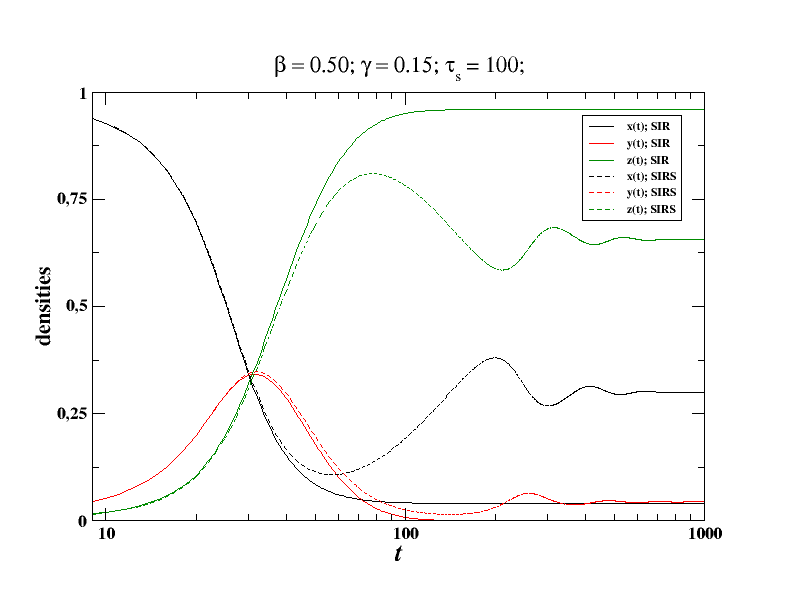
\includegraphics[width=91mm]{Fig1.png}
  \caption{Comparison between SIR and SIRS models: the possibility for recovered individuals to get susceptible again, though at a very slow time scale, changes dramatically the behaviour of the system. The abscissa axis is in logarithmic scale to make the dynamics clearer.}
  \label{fig1}
\end{figure}

\ 

\section{Stochastic SIRS Model}

The model(s) sketched in the previous section assume the mean field approximation, that is, the individuals composing the population are thought uniformly distributed in space, and totally connected among themselves (or, equivalently, each individual interacts with everyone else with the same frequency). More subtly, also the main features of the epidemics are considered uniformly distributed: the parameters $\beta$, $\gamma$ and $\tau_s$ are exactly the same for each agent and each interaction. This is a very strong assumption which does not take into account the usually large variability through the population. In particular, let us focus on the infection rate $\beta$: it depends on several factors: the capability of an infected person to transmit the pathogen, the probability of a susceptible individual to get infected, the real rate of interaction between an infected and a susceptible people, etc. 

Contrarily to the other two parameters, $\beta$ does not depend only on the physical and biological properties of pathogen and humans, but also on the behaviour of the people. Indeed, the infection rates will be influenced also by how much, say, subjects respect norms on social distance, if they are susceptible or infected but asymptomatic, on quarantine if infected, and so on. In general, this introduces a variability on the parameter $\beta$, which cannot be considered a constant and uniform number anymore: therefore, it is straight forward to modify Eqs.~(\ref{sirs}) by considering a stochastic variable $\xi_\beta$ instead of the classical infection rate:

\begin{equation}
\left\{
\begin{array}{l}
\dot x = -\xi_\beta(t) xy + \frac{1}{\tau_s}z\\
\ \\
\dot y = \xi_\beta(t) xy -\gamma y \\
\ \\
\dot z = \gamma y - \frac{1}{\tau_s}z \ ,
\end{array}
\right.
    \label{stoch}
\end{equation}

\noindent where it has to be specified the probability distribution of $\xi_\beta$, which of course will assume in general different values at different times.

There are obviously infinite possible distributions from which we could extract $\xi_\beta$: the point here is to choose the right one which describes the variability of norm complying by people and is realistic enough allowing us to draw some useful conclusions. In the next subsection I will start to make some general considerations about it, and write down a toy model just to depict the consequences of this refinement of the model with respect to the deterministic one.

\subsection*{The role of Social Norms}

In the current situation, many countries have declared several measures aiming at reducing contacts among people and thus the infection rate. Such measures go from mild ones to the hardest, as the lock-down of whole regions or countries. Unfortunately (and predictably), the efficacy of these policies on social distance, gathering, traffic flows etc. is heavily conditioned by the rate of compliance of the citizens, being the countries which have weaker social norms about the respect of the laws may encounter difficulties.

Just to get a preliminary idea about the possible consequences of lacking in social norms complying, I tested a rough, naive version of stochastic SIRS model. In details, I implemented it as follows: at every elementary integration step, the infection rate is picked as

\begin{equation}
\xi_\beta(t)=
\left\{
\begin{array}{lcl}
\beta & \ \ \  & \mbox{with probability $1-p$} \\
\ & \ & \ \\
(N-1)\ \eta(t) & \ \ \  & \mbox{with probability $p$} \ ; 
\end{array}
\right.
    \label{st_b}
\end{equation}

\ 

\noindent where $\beta$ is the baseline infection rate, $p\in[0,1]$ and $N\in\mathbb{N}$ are fixed parameters, and $\eta(t)$ is a random number extracted by a uniform distribution among 0 and 1. The factor $(N-1)$ instead of $N$ is a relic of my first idea, where an infected agent could in principle meet and transmit the virus to at most $N-1$ other people, given $N$ the total population. In this toy model only aimed to visualize the main differences with its deterministic version, anyway, it lost this meaning.

In Figures~\ref{fig2} and ~\ref{fig3} we show few comparisons among the different versions of the model (SIR and SIRS, both deterministic and stochastic). As it is easy to see, the stochasticity changes deeply the dynamics and final fate of the system. First of all, in general it increases the maximum density of infected people, similarly to the removing the immunization after recovery. More dramatically, as shown in Fig.~\ref{fig3}, in some cases it shifts the system from a final total recovery to an equilibrium with finite rate of infected, that is, at individual level, subjects alternate their status from susceptible to infected to recovered to susceptible again and so on.

\begin{figure}
  \centering
  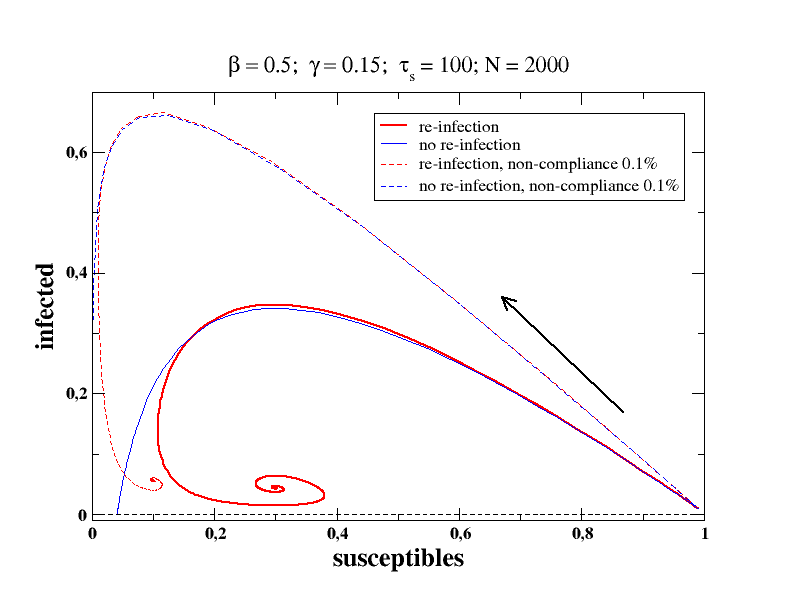
\includegraphics[width=91mm]{Fig2.png}
  \caption{Comparison among deterministic SIR and SIRS models (constant $\beta$), stochastic SIR and SIRS models (random $\xi_\beta$) by means of the orbit susceptible-infected. The non-compliance rate of $0.1\%$ is the parameter $p=0.001$. The remaining parameter values are indicated above the graphics, the arrow shows the time direction. For the stochastic model, results averaged over 200 independent realizations. The main difference here is the maximum value of infected people density, much higher in the stochastic case.}
  \label{fig2}
\end{figure}

\ 

\begin{figure}
  \centering
  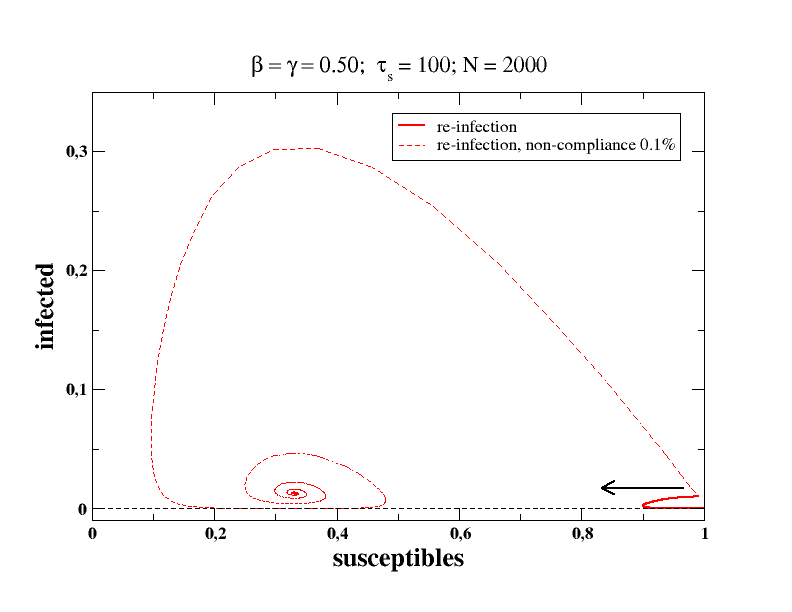
\includegraphics[width=91mm]{Fig3.png}
  \caption{Comparison among stochastic SIR and SIRS models (random $\xi_\beta$), analogously to Fig.~\ref{fig2}. Differently from the case of Fig.~\ref{fig2}, here the values of $\beta$ and $\gamma$ are such that the behaviour of the two models are especially different (the remaining parameters have the same value): the deterministic ends up with a population totally safe and sound, the stochastic one in a mixed (active) equilibrium with the coexistence of susceptible, infected and recovered individuals; moreover, the maximum density of infected people density is pretty high.}
  \label{fig3}
\end{figure}

In analytical terms, we could think that the stochastic model works as the deterministic SIRS given by Eqs.~(\ref{sirs}), but with an average infection rate which is, in the limit of small $p$ and large $N$,  

$$
\langle\xi_\beta\rangle = \beta+\frac{pN}{2} \ , 
$$

\noindent but unfortunately this does not seem to be the case: indeed, a deterministic SIRS model with a shifted infection rate $\beta\rightarrow\beta'=\beta+(pN)/2$ does not behave as the correspondent stochastic version.

\ 

\section{Agent-based approach}

Up to now, I have just played with simple models in order to understand them better and pave the way for next, accurate analyses. The main goal of our work is to study the dynamics of social norms in human societies and the present emergency with its consequences is a good chance to catch it in real life. This can potentially help us to improve the models, set their parameters and make them useful for (at least partial) reliable predictions. To this aim, the first step is to go beyond a mere analytical approach towards simulations by means of agent-based models (ABMs). With ABMs, it is possible to enrich the baseline model much more easily.

\subsubsection*{Plan for next steps:} First of all, build on my own an SIRS ABM, as a starting point. Once we have it, adding ingredients, as for example the following ones:

\begin{itemize}
    \item besides the susceptible-infected-recovered kinds of agents (which each individual can belong to during the dynamics), it will be possible to define different species of agents: the ones which comply the norms, the ones which comply less or do not comply at all, etc; an agent of a given species in general gets infected/recovered differently from others.
    \item This categorization represents the internal mental state of the individuals, and does not evolve in time or, but if it does, evolves through a different dynamics, which can be inserted in the ABM.
    \item the rates of the SIRS model themselves can change in time, for both external or internal motivations, and can distributed through the population in different ways.
    \item the influence of media, institutions, opinion leaders etc. can be taken into account.
    \item In general, well-known models of opinion and behavioural dynamics can be merged with the ABM.
    \item Fitting the values of the model parameters with real data will be much more easy.
    \item Whatever else can be useful to make model more realistic.
\end{itemize}

Of course, a similar road map can be write down and accomplished starting from any baseline model besides SIRS, if necessary. I stress the fact that my present goal is not to fight against the CoVid-19 pandemic, but the understanding of the human behaviour in this situation. The simulation results, together with experiments and observations will be surely useful for the next emergencies.

\ 

%\newpage 
\begin{thebibliography}{50}

\bibitem{mar20}
Up to today, April 2, only in the arXiv 264 preprints, come out in 2020, have "COVID-19" or "CoVid-19" in their title and/or abstract. A graphics showing the increasing of research in epidemics after the outbreak of the pandemics, up to the end of February, can be found at
\newline https://medium.com/@tomaspueyo/coronavirus-the-hammer-and-the-dance-be9337092b56 (chart 10).

\bibitem{gon11}
Gon\c{c}alves, Sebasti\'an, Guillermo Abramson, and Marcelo FC Gomes. "Oscillations in SIRS model with distributed delays." The European Physical Journal B 81.3 (2011): 363.

\bibitem{ker27}
Kermack, William Ogilvy, and Anderson G. McKendrick. "A contribution to the mathematical theory of epidemics." Proceedings of the royal society of london. Series A, Containing papers of a mathematical and physical character 115.772 (1927): 700-721.

\bibitem{ves20}
Chinazzi, Matteo, et al. "The effect of travel restrictions on the spread of the 2019 novel coronavirus (COVID-19) outbreak." Science (2020).

\bibitem{che20}
Chen, Wen-Hsiang, et al. "The SARS-CoV-2 Vaccine Pipeline: an Overview." Current Tropical Medicine Reports (2020): 1-4. See also: https://youtu.be/SzckrIwDeI0 (in italian).

\end{thebibliography}

\end{document}
